\documentclass{beamer}

\title{Brancher AnyBlok à 14 ans d'historique métier}
\subtitle{Une histoire terrifiante de PHP, MySQL et MsSQL}
\author{Jean-Sébastien SUZANNE et Hugo QUEZADA}
\date{2 novembre 2019}

\newcommand{\TwitterLogo}{\protect
\includegraphics[height=
1.7ex,keepaspectratio]{./twitter.png}}
\newcommand{\EmailLogo}{\protect
\includegraphics[height=
1.7ex,keepaspectratio]{./email.png}}
\newcommand{\AnyBlokLogo}{\protect
\includegraphics[height=
1.7ex,keepaspectratio]{./anyblok.png}}

\usepackage{hyperref}
\usepackage{color}

\usetheme{Amsterdam}
\begin{document}
	\frame {
		\titlepage
	}
	
	\frame {
		\frametitle{Qui sommes nous ?}
		
		\begin{columns}
            \begin{column}{3cm}
                \begin{figure}
  					
\includegraphics[width=\linewidth]{logosensee-carre.jpg}
  					\label{fig:sensee}
				\end{figure}
			\end{column}
			\begin{column}{3cm}
				\begin{figure}
  					
\includegraphics[width=\linewidth]{lentillesmoinscheres-mobile.png}
  					\label{fig:lmc}
				\end{figure}
			\end{column}
		\end{columns} 			
		\begin{columns}
            \begin{column}{5cm}
                \textbf{\AnyBlokLogo{} Jean-Sébastien Suzanne}
		    	\begin{itemize}
			  		\item Répond aussi au nom de PAPABLOK
			  		\item \TwitterLogo{} @jssuzanne
			    	\item \EmailLogo{} js.suzanne@sensee.com
		    	\end{itemize}
			\end{column}
			\begin{column}{5cm}
				\textbf{Hugo Quezada}
		    	\begin{itemize}
			  		\item Répond seulement au nom de Hugo
			  		\break
			    	\item \EmailLogo{} h.quezada@sensee.com
		    	\end{itemize}
			\end{column}
		\end{columns}
	}
	\frame{
		\begin{center}
			{\color{anyblok}\huge{Existant}}
		\end{center}
		\begin{center}
			
\includegraphics[width=10ex]{php.jpeg}
			
\includegraphics[width=10ex]{mysql.png}
			
\includegraphics[width=10ex]{mssql.jpeg}
		\end{center}
	}
	\frame{
		\frametitle{14 ans de code...}
		\framesubtitle{Existant}
		\begin{itemize}
			\item Code legacy en PHP5 (pas de troll SVP)
			\item Pas de framework, beaucoup de code, très peu d'objet
			\break
			\pause
			\begin{columns}
				\begin{column}{4cm}
					\item Pas de tests
					\item Pas de CI
					\break
					\pause
					\item Pas d'ORM
				\end{column}
				\begin{column}{3.5cm}
					\pause
					
\includegraphics[width=20ex]{crying_trollface.jpeg}
				\end{column}
			\end{columns}
		\end{itemize}
	}
	
	\frame{
		\frametitle{Une BdD un peu complexe...}
		\framesubtitle{Existant}
		\begin{itemize}
			\item  Schémas de base de données multiples
			\pause
			\item  Écosystème avec plusieurs SGBD (MySQL, MsSQL) souvent sans API
			\begin{figure}[p]
				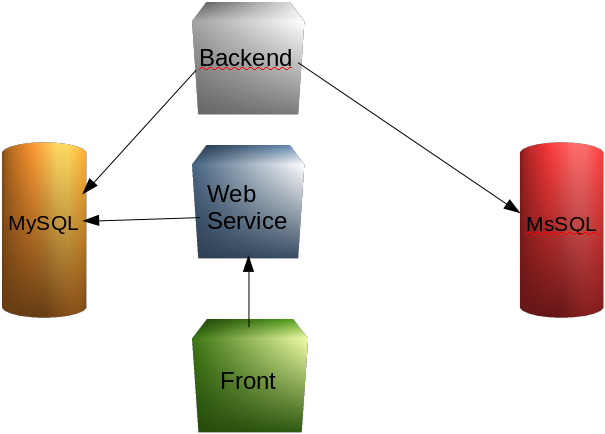
\includegraphics[height=25ex,keepaspectratio]{./schema_simplifie_lmc.png}
				\caption{Schéma simplifié}
			\end{figure}
		\end{itemize}
	}
	\frame{
		\begin{center}
			{\color{anyblok}\huge{Vision finale}}
		\end{center}
		\begin{center}
			
\includegraphics[width=10ex]{python.png}
			
\includegraphics[width=10ex]{anyblok.png}
			
\includegraphics[width=10ex]{sqlalchemy.png}
			
\includegraphics[width=10ex]{pyramid.png}
		\end{center}

	}
	\frame{
		\frametitle{L'objectif}
		\framesubtitle{Vision finale}
		\begin{itemize}
		    \item Un code python propre et testé
			\item Une API simple et uniforme, utilisé dans tous nos projets
			\item Une application plus proche des standards actuels
			\item Un projet plus séduisant et plus attrayant pour des potentiels futurs développeurs 
		\end{itemize}
	}
	\frame{
		\frametitle{La stratégie}
		\framesubtitle{Vision finale}
		\begin{itemize}
			\item Modèle d'étranglement (Strangle pattern)
			\begin{figure}[p]
				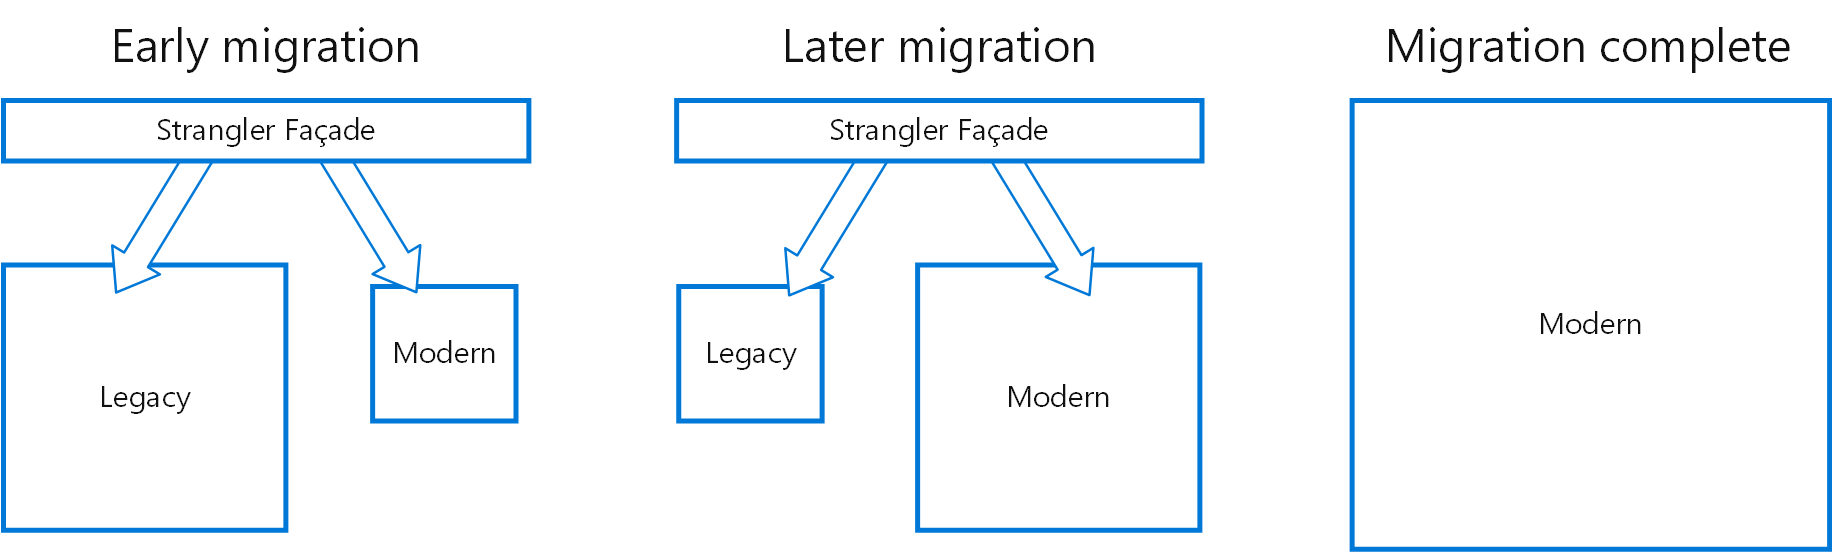
\includegraphics[height=15ex,keepaspectratio]{./strangler.png}
			\end{figure}
			\item Mapping des tables avec un nommage plus clair
			\item Développement piloté par les tests (TDD)
		\end{itemize}
	}
	\frame{
		\begin{center}
			{\color{anyblok}\huge{Pourquoi avoir choisi AnyBlok ?}}
		\end{center}
		\begin{center}
			
\includegraphics[width=10ex]{anyblok.png}
		\end{center}
	}
	\frame{
		\frametitle{AnyBlok: Présentation}
		\framesubtitle{Pourquoi avoir choisi AnyBlok ?}
		\begin{itemize}
		\item Python 3.6 et plus
		\item MPL2
		\item PyPi
		\item Modulaire
		\item Dépendances fiables (SQLAlchemy, Alembic, ...)
		\item Possibilité de reprendre une base existante.
		\end{itemize}
	}
	\frame{
		\frametitle{AnyBlok: Structure}
		\framesubtitle{Pourquoi avoir choisi AnyBlok ?}
		\begin{figure}
  			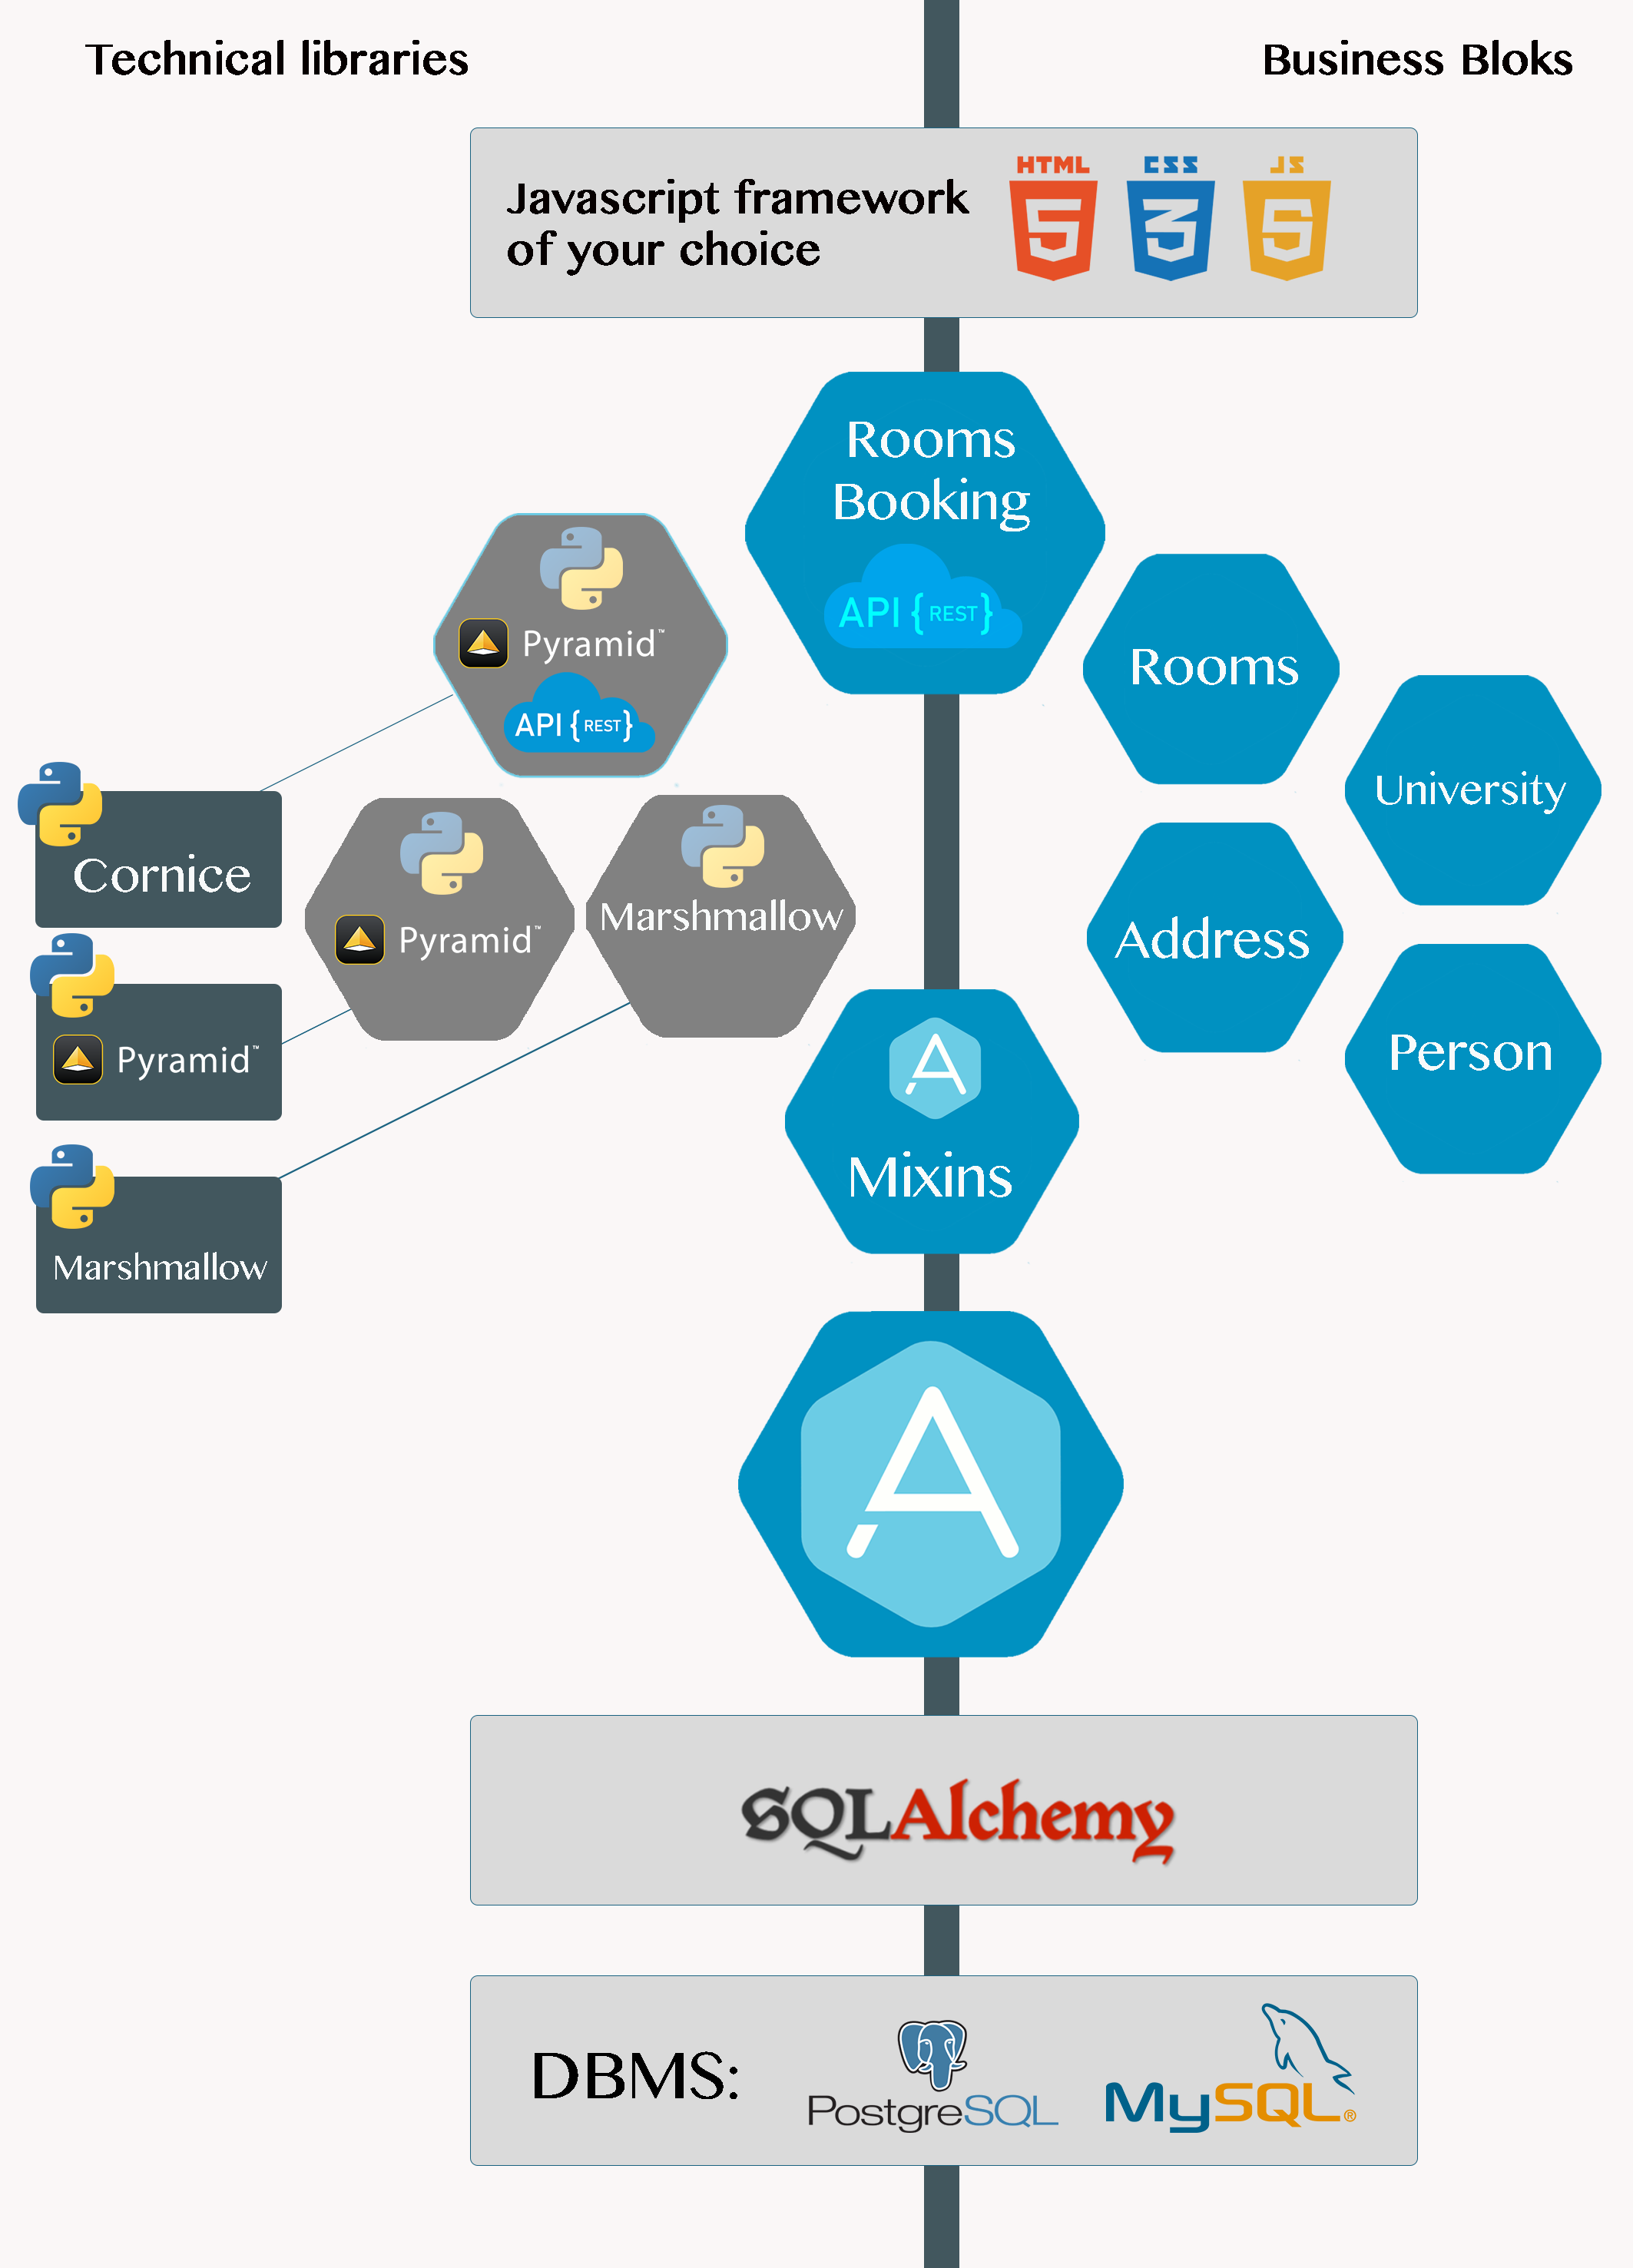
\includegraphics[height=42ex,keepaspectratio]{bloks_dependencies.png}
  			\label{fig:test unitaire}
		\end{figure}
	}
	\frame{
		\frametitle{AnyBlok: Écrire des tests pour notre Model}
		\framesubtitle{Pourquoi avoir choisi AnyBlok ?}
		\begin{figure}
  			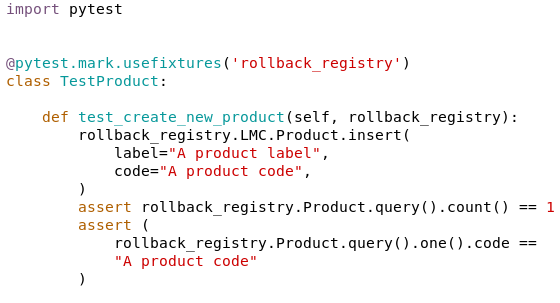
\includegraphics[width=\linewidth]{testU.png}
  			\label{fig:test unitaire}
		\end{figure}
	}
	\frame{
		\frametitle{AnyBlok: Définir le Model}
		\framesubtitle{Pourquoi avoir choisi AnyBlok ?}
		\begin{figure}
  			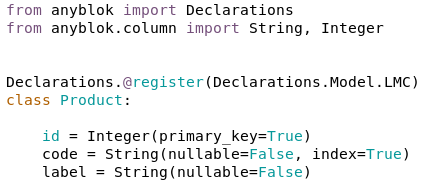
\includegraphics[width=\linewidth]{model1.png}
  			\label{fig:Model 1}
		\end{figure}
	}
	\frame{
		\frametitle{AnyBlok: Définir un Model sur une table existante}
		\framesubtitle{Pourquoi avoir choisi AnyBlok ?}
		\begin{figure}
  			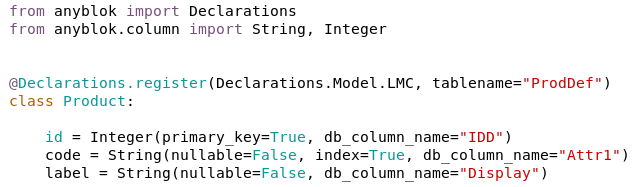
\includegraphics[width=\linewidth]{model2.png}
  			\label{fig:Model 2}
		\end{figure}
	}
	\frame{
		\frametitle{AnyBlok: Écrire des tests pour notre API}
		\framesubtitle{Pourquoi avoir choisi AnyBlok ?}
		\begin{figure}
  			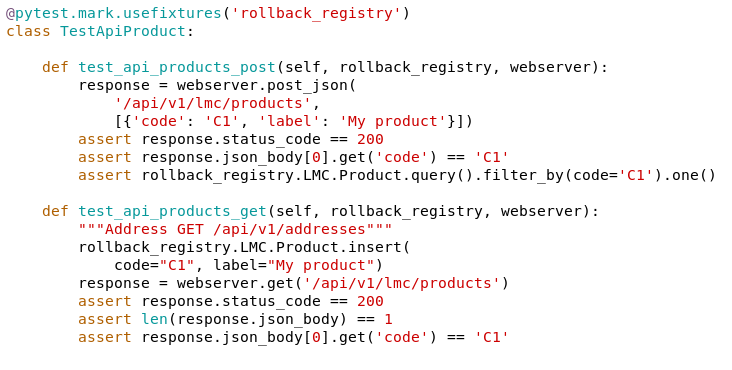
\includegraphics[width=\linewidth]{apitestU.png}
  			\label{fig:test unitaire API}
		\end{figure}
	}
	\frame{
		\frametitle{AnyBlok: Écrire une API REST}
		\framesubtitle{Pourquoi avoir choisi AnyBlok ?}
		\begin{figure}
  			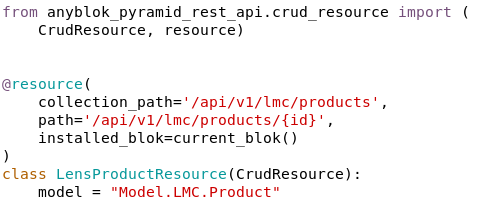
\includegraphics[width=\linewidth]{api.png}
  			\label{fig: API}
		\end{figure}
	}
	\frame{
		\begin{center}
			{\color{anyblok}\huge{Évolutions et intégrations dans AnyBlok}}
		\end{center}
	}
	\frame{
		\frametitle{Compatibilité avec MySQL}
		\framesubtitle{Évolutions et intégrations dans AnyBlok}
		\begin{itemize}
			\item Deux semaines de travail
			\item Beaucoup de recherches et d'incompréhensions 
		\end{itemize}
	}	
	\frame{
		\frametitle{Compatibilité avec MySQL : Les tests unitaires}
		\framesubtitle{Évolutions et intégrations dans AnyBlok}
		\begin{itemize}
			\item Mise à jour de la configuration Travis-CI
			\item Activer le mode transactionnel de innoDB
			\item {\color{blue}\href{https://dev.mysql.com/doc/refman/8.0/en/implicit-commit.html}{Les commits implicites}}
		\end{itemize}
	}	
	\frame{
		\frametitle{Compatibilité avec MySQL : Limitations}
		\framesubtitle{Évolutions et intégrations dans AnyBlok}
		\begin{itemize}
			\item Pas de Python 3.5
			\item Contrainte exclusive à PostgreSQL
			\item Datetime naïves
			\item Pas de chiffrement sur les colonnes de type UUID
			\item Pas de véritable Booléen
		\end{itemize}
	}	
	\frame{
		\frametitle{Compatibilité avec MariaDB : Limitations }
		\framesubtitle{Évolutions et intégrations dans AnyBlok}
		\begin{itemize}
			\item Pas de Python 3.5
			\item Contrainte exclusive à PostgreSQL
			\item Datetime naïves
			\item Pas de chiffrement sur les colonnes UUID
			\item Pas de véritable Booléen
			\item \pause Taille des clés primaires plus petite
			\item Pas de colonnes JSON
		\end{itemize}
	}
	\frame{
		\frametitle{Compatibilité avec MsSQL : Limitations}
		\framesubtitle{Évolutions et intégrations dans AnyBlok}
		\begin{itemize}
			\item Pas de Python 3.5
			\item Contrainte exclusive à PostgreSQL
			\item \pause Lent... Très très lent...
		\end{itemize}
	}
	\frame{
		\frametitle{Définition de schémas}
		\framesubtitle{Évolutions et intégrations dans AnyBlok}
		Choix :
		\begin{itemize}
			\item Programmatique ou par configuration
			\item Poser sur un modèle ou un namespace
			\item Ajout de suffixes ou préfixes pour les tests
		\end{itemize}
		\hfill \linebreak
		\pause Problématiques :
		\begin{itemize}
			\item Génération de foreign key
			\item Migration
		\end{itemize}
	}
	\frame{
		\frametitle{Lier un Model à un schéma}
		\framesubtitle{Évolutions et intégrations dans AnyBlok}
		Dans le Model :
		\begin{figure}
  			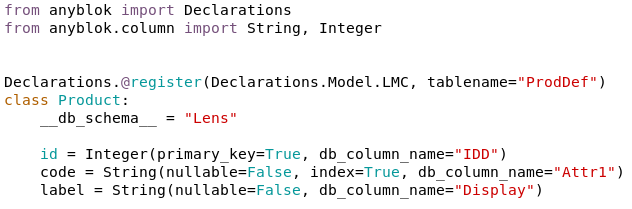
\includegraphics[width=\linewidth]{schema.png}
  			\label{fig:Model avec un schema}
		\end{figure}
		Par la configuration :
		\begin{figure}
  			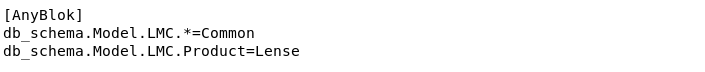
\includegraphics[width=\linewidth]{schema2.png}
  			\label{fig:Schema depuis la conf}
		\end{figure}
	
	}
	\frame{
		\begin{center}
			
\includegraphics[height=42ex,keepaspectratio]{logo-furetui.png}
		\end{center}
	}
	\frame{
		\frametitle{Interface Graphique}
		\framesubtitle{FuretUI}
		\begin{figure}

  			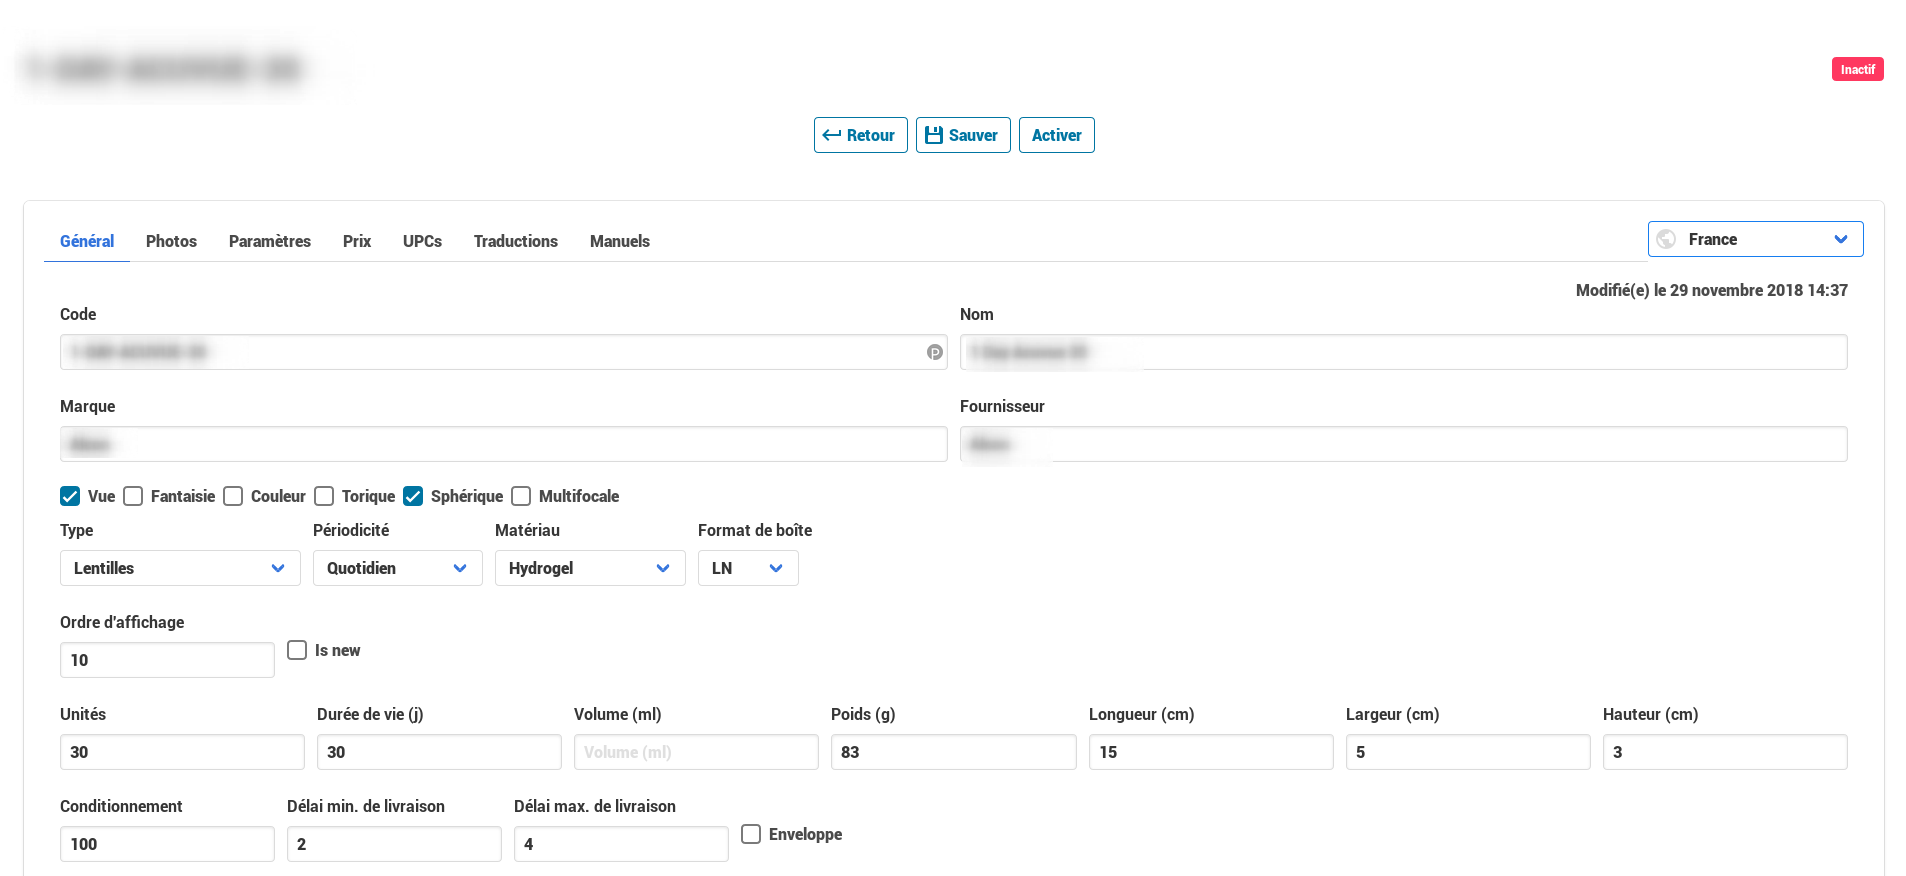
\includegraphics[width=\linewidth]{exemple_furetui_produits.png}
  			\label{fig: FuretUI List}
		\end{figure}
	}
	\frame{
		\frametitle{Interface Graphique}
		\framesubtitle{FuretUI}
		\begin{figure}
  			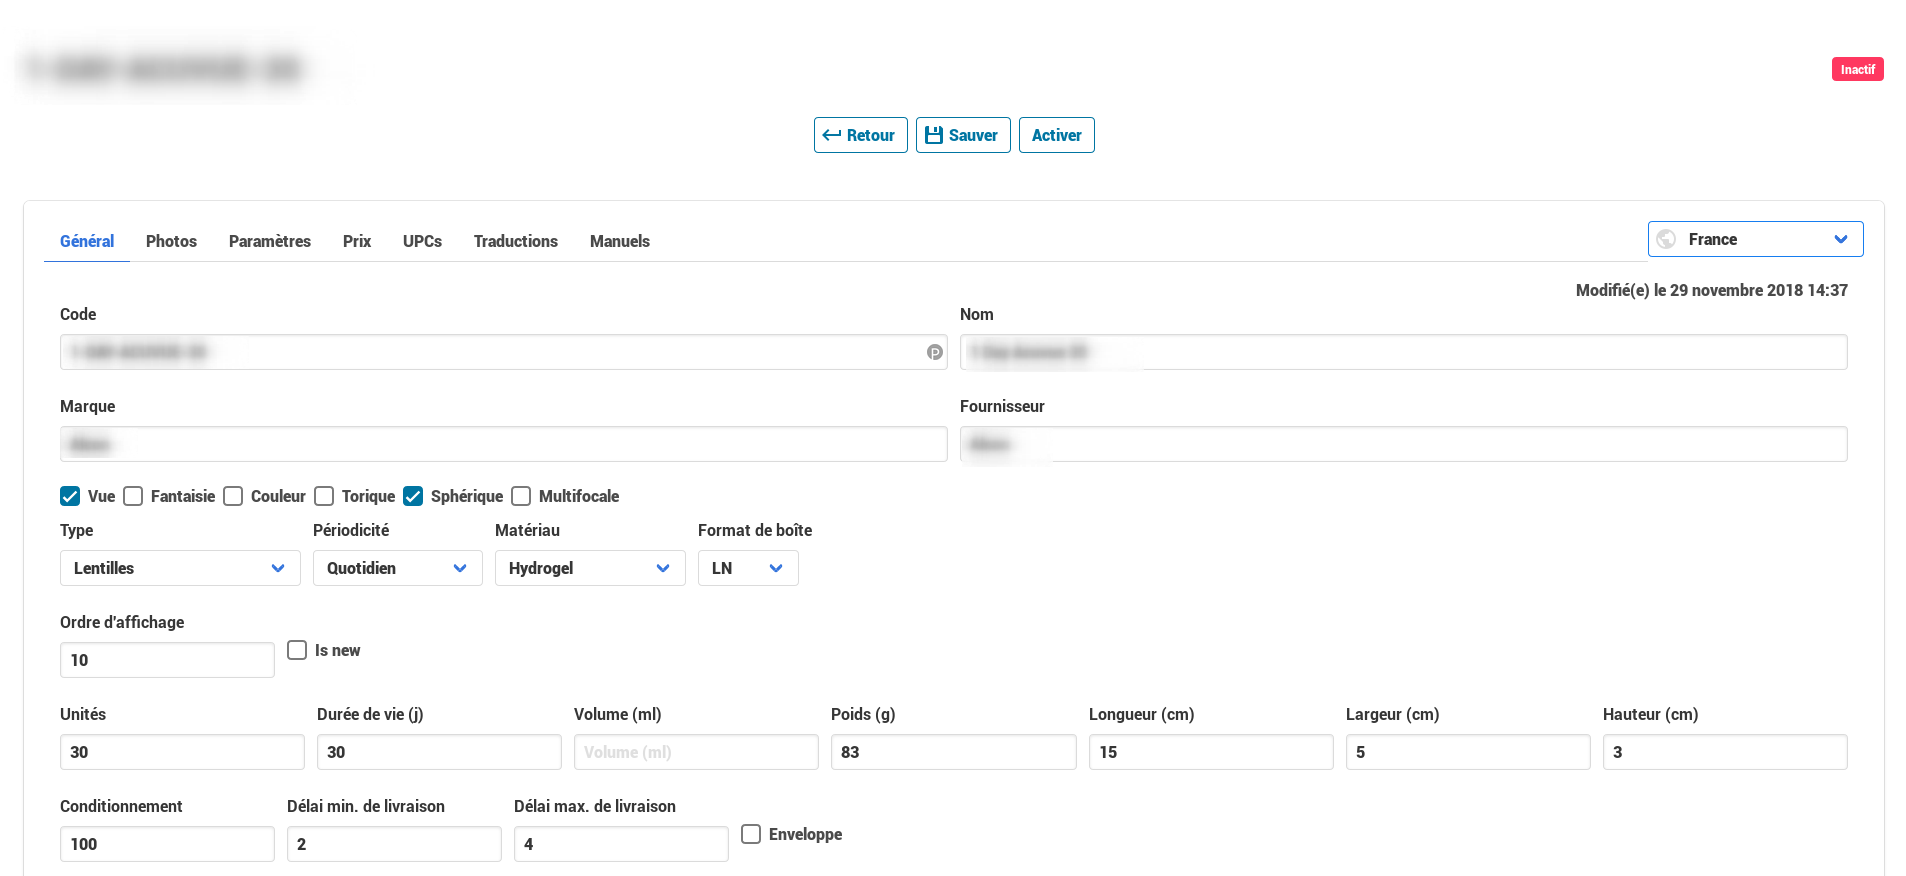
\includegraphics[width=\linewidth]{exemple_furetui_produits_page.png}
  			\label{fig: FuretUI Page}
		\end{figure}
	}
	\frame{
		\frametitle{AnyBlok}
		\framesubtitle{Documentation}
		\begin{itemize}
		\item https://anyblok.gitbooks.io/anyblok-book/content/en/
		\item https://doc.anyblok.org
		\item https://github.com/AnyBlok
		\item https://gitter.im/AnyBlok/community
		\end{itemize}
	}
	\frame{
		\begin{center}
			{\color{anyblok}\huge{MERCI !}}
		\end{center}
	}
	\frame{
		\begin{center}
			{\color{anyblok}\huge{Avez-vous des questions ?}}
		\end{center}
	}
\end{document}
